\documentclass[border=10pt]{standalone}

\usepackage{tikz}
\usepackage{tikzsymbols}
\usetikzlibrary{calc,patterns,shapes.geometric}

\def\centerarc[#1](#2)(#3:#4:#5){\draw[#1] ($(#2)+({#5*cos(#3)},{#5*sin(#3)})$) arc (#3:#4:#5);}

\begin{document}
	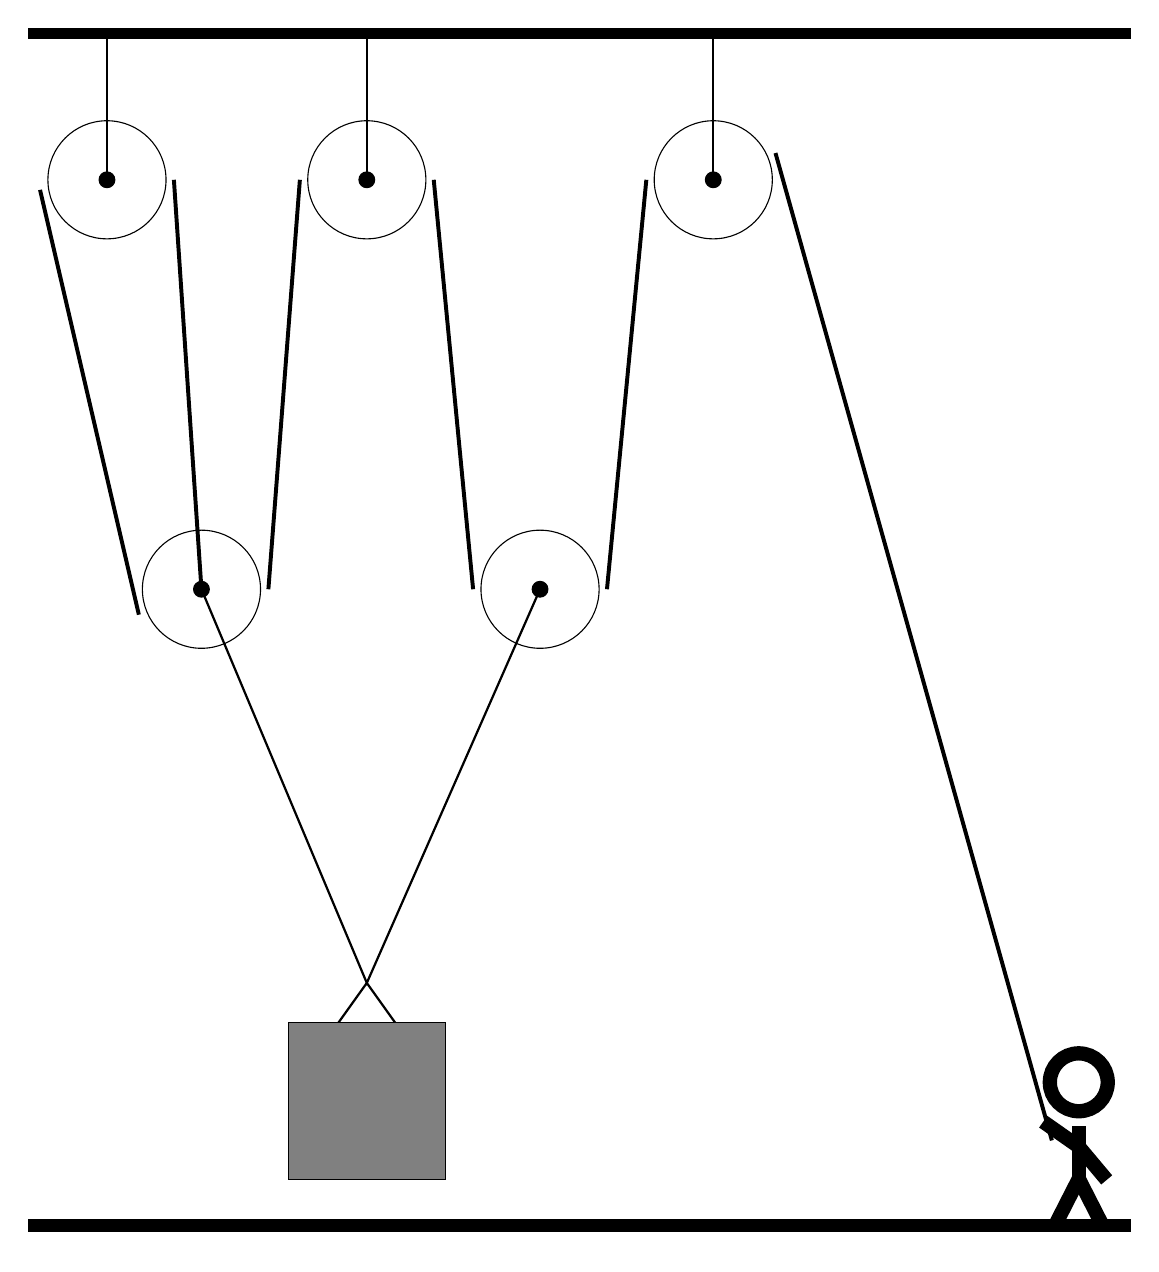
\begin{tikzpicture}
		%%%%% START %%%%%
		\draw[fill=black] (-2, 12) rectangle (12, 12.125);
		
		\draw (-1, 10.2) circle (0.75);
		\draw[fill=black] (-1, 10.2) circle (0.1);
		\draw[thick] (-1, 10.2) -- (-1, 12);
		
		\draw (2.3, 10.2) circle (0.75);
		\draw[fill=black] (2.3, 10.2) circle (0.1);
		\draw[thick] (2.3, 10.2) -- (2.3, 12);
		
		\draw (6.7, 10.2) circle (0.75);
		\draw[fill=black] (6.7, 10.2) circle (0.1);
		\draw[thick] (6.7, 10.2) -- (6.7, 12);
		
		\draw (0.2, 5) circle (0.75);
		\draw[fill=black] (0.2, 5) circle (0.1);
		
		\draw (4.5, 5) circle (0.75);
		\draw[fill=black] (4.5, 5) circle (0.1);
		
		\draw[thick] (0.2, 5) -- (2.3, 0)  -- (4.5, 5);
		\draw[thick]  (1.8, -0.7) -- (2.3, 0) -- (2.8, -0.7);
		\draw[fill=black!50] (1.3, -0.5) rectangle (3.3, -2.5);
		
		\draw[line width=0.5mm] (0.2, 5) -- (-0.15, 10.2);
		\centerarc[line width=0.5mm](-1, 10.2)(0:200:0.85);
		\draw[line width=0.5mm] (-1.85, 10.072) -- (-0.595, 4.677);
		\centerarc[line width=0.5mm](0.2, 5)(200:360:0.85);
		\draw[line width=0.5mm](1.05, 5) -- (1.45, 10.2);
		\centerarc[line width=0.5mm](2.3, 10.2)(0:180:0.85);
		\draw[line width=0.5mm] (3.15, 10.2) -- (3.65, 5);
		\centerarc[line width=0.5mm](4.5, 5)(180:360:0.85);
		\draw[line width=0.5mm] (5.35, 5) -- (5.85, 10.2);
		\centerarc[line width=0.5mm](6.7, 10.2)(20:180:0.85);
		\draw[line width=0.5mm](7.49, 10.54)  -- (11, -2);
		
		\node at (11.3, -2) {\Strichmaxerl[10][-35][-50]};
		
		\draw[fill=black] (-2, -3) rectangle (12, -3.15);
		%%%%% END %%%%%
	\end{tikzpicture}
\end{document}